\documentclass{ximera}
\input{../preamble}
\addPrintStyle{..}
\begin{document}
\author{Alexander Holvoet}
\xmtitle{Matrixtransformaties}{}

% Oefeningen: Matrixtransformaties voor letterfonts
% Gebaseerd op "N" transformatie probleem en Pat & Jamie samenwerking

\begin{problem}
Veronderstel dat de letter ``N'' aan de linkerkant geschreven is in een regulier 12-punts lettertype. Vind een matrix $A$ die de ``N'' transformeert naar de letter aan de rechterkant, die geschreven is in cursief (italic) 16-punts lettertype.

\begin{center}
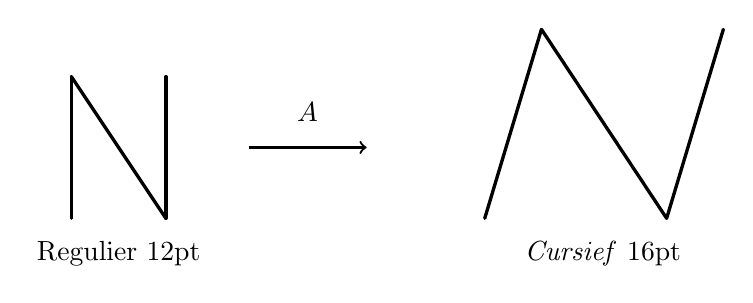
\begin{tikzpicture}[scale=1.5]
% Reguliere N (12-punts, schaal 1)
\begin{scope}
\draw[very thick, line cap=round] (0,0) -- (0,1.2);
\draw[very thick, line cap=round] (0,1.2) -- (0.8,0);
\draw[very thick, line cap=round] (0.8,0) -- (0.8,1.2);
\node at (0.4,-0.3) {Regulier 12pt};
\end{scope}

% Pijl
\draw[->, thick] (1.5,0.6) -- (2.5,0.6);
\node at (2,0.9) {$A$};

% Cursieve N (16-punts met shear, schaal 4/3)
\begin{scope}[xshift=3.5cm]
\draw[very thick, line cap=round] (0,0) -- (0.48,1.6);
\draw[very thick, line cap=round] (0.48,1.6) -- (1.54,0);
\draw[very thick, line cap=round] (1.54,0) -- (2.02,1.6);
\node at (1,-0.3) {\textit{Cursief} 16pt};
\end{scope}
\end{tikzpicture}
\end{center}

$$A = \begin{pmatrix} \phantom{00} & \phantom{00} \\ \phantom{00} & \phantom{00} \end{pmatrix}$$

Werk met een kleine groep en schrijf jullie oplossing en aanpak uit. Maak een lijst van eventuele aannames die jullie maken, of eventuele vragen voor verdere uitwerking die bij jullie opkomen.
\end{problem}

\begin{freeResponse}
\textbf{Conceptuele aanpak:} We moeten een matrix vinden die twee transformaties combineert:
\begin{enumerate}
\item Schaling van 12-punts naar 16-punts (factor $\frac{16}{12} = \frac{4}{3}$)
\item Schuintrekken ('shear') voor het cursieve effect
\end{enumerate}

\textbf{Stapsgewijze oplossing:}

\textbf{Stap 1: Schaling}
Om van 12-punts naar 16-punts te gaan, schalen we met factor $\frac{4}{3}$:
$$S = \begin{pmatrix} 4/3 & 0 \\ 0 & 4/3 \end{pmatrix}$$

\textbf{Stap 2: Schuintrekking (shear)}
Voor het cursieve effect gebruiken we een horizontale shear. Een typische cursieve hoek is ongeveer 15°, wat overeenkomt met $\tan(15°) \approx 0.27$. We gebruiken een shear parameter van ongeveer $0.3$:
$$H = \begin{pmatrix} 1 & 0.3 \\ 0 & 1 \end{pmatrix}$$

\textbf{Stap 3: Compositie}
De totale transformatie is het product (let op volgorde!):
$$A = H \cdot S = \begin{pmatrix} 1 & 0.3 \\ 0 & 1 \end{pmatrix} \begin{pmatrix} 4/3 & 0 \\ 0 & 4/3 \end{pmatrix} = \begin{pmatrix} 4/3 & 2/5 \\ 0 & 4/3 \end{pmatrix}$$

of in decimalen:
$$A \approx \begin{pmatrix} 1.33 & 0.40 \\ 0 & 1.33 \end{pmatrix}$$

\textbf{Aannames:}
\begin{itemize}
\item De cursieve hoek is ongeveer 15° (dit kan variëren per lettertype)
\item We schalen uniform in beide richtingen (sommige fonts hebben verschillende x- en y-schaling)
\item De oorsprong ligt aan de basis van de letter
\item Er is geen rotatie component
\end{itemize}

\textbf{Verificatie:}
Test met een punt uit de ``N'', bijvoorbeeld de rechterbovenhoek:
\begin{itemize}
\item Voor: $(1, 1)$ in 12-punts
\item Na: $A \begin{pmatrix} 1 \\ 1 \end{pmatrix} = \begin{pmatrix} 1.73 \\ 1.33 \end{pmatrix}$
\item De letter is hoger én naar rechts verschoven (cursief effect)
\end{itemize}

\textbf{Mogelijke studentenfouten:}
\begin{itemize}
\item Alleen schalen, het cursieve effect vergeten
\item Verkeerde volgorde van transformaties (eerst shear, dan schalen vs. omgekeerd)
\item Verkeerde shear richting (verticaal in plaats van horizontaal)
\item Schalen met 16 in plaats van $\frac{16}{12}$
\item Minteken fout in de shear matrix
\end{itemize}
\end{freeResponse}

\begin{problem}
Vorig semester beschreven twee eerstejaars lineaire algebra studenten---Pat en Jamie---hun aanpak voor het bovenstaande probleem. Lees hun beschrijving hieronder.

\begin{quote}
\textit{``Om de matrix $A$ te vinden, gaan we een matrix vinden die de langere ``N'' maakt (van 12-punts naar 16-punts), een matrix vinden die de kortere ``N'' schuintrekt, en dan het product van die twee vinden om de gewenste matrix $A$ te krijgen.''}
\end{quote}

Denk je dat hun aanpak hen in staat stelde om een matrix $A$ te vinden? Lijkt het verstandig? Zo ja, denk je dat het dezelfde matrix $A$ is die we in het vorige probleem vonden?
\end{problem}

\begin{freeResponse}
\textbf{Analyse van Pat en Jamie's aanpak:}

\textbf{Antwoord:} Ja, hun aanpak is verstandig en zou moeten werken! Het is in essentie dezelfde aanpak als in het vorige probleem.

\textbf{Waarom het werkt:}
\begin{itemize}
\item Ze decomponeren een complexe transformatie in eenvoudiger stappen (schaling en shear)
\item Ze herkennen dat matrixvermenigvuldiging transformaties componeert
\item Hun redenering toont begrip van het principe van transformatie-compositie
\end{itemize}

\textbf{Vergelijking met vorige oplossing:}
Pat en Jamie's aanpak is identiek aan de aanpak in het vorige probleem:
\begin{enumerate}
\item Schaalmatrix $S$: van 12-punts naar 16-punts
\item Shear matrix $H$: voor cursief effect
\item Product $A = H \cdot S$ (of $A = S \cdot H$, afhankelijk van volgorde)
\end{enumerate}

\textbf{Belangrijke overweging - volgorde van transformaties:}

Er zijn twee mogelijke volgordes:

\textbf{Optie 1:} Eerst schalen, dan shear: $A = H \cdot S$
$$A = \begin{pmatrix} 1 & 0.3 \\ 0 & 1 \end{pmatrix} \begin{pmatrix} 4/3 & 0 \\ 0 & 4/3 \end{pmatrix} = \begin{pmatrix} 4/3 & 2/5 \\ 0 & 4/3 \end{pmatrix}$$

\textbf{Optie 2:} Eerst shear, dan schalen: $A = S \cdot H$
$$A = \begin{pmatrix} 4/3 & 0 \\ 0 & 4/3 \end{pmatrix} \begin{pmatrix} 1 & 0.3 \\ 0 & 1 \end{pmatrix} = \begin{pmatrix} 4/3 & 2/5 \\ 0 & 4/3 \end{pmatrix}$$

In dit specifieke geval geven beide volgordes hetzelfde resultaat! Dit komt omdat:
\begin{itemize}
\item De schaling uniform is (zelfde factor in $x$ en $y$)
\item De shear alleen horizontaal is
\item Uniforme schaling commuteert met horizontale shear
\end{itemize}

\textbf{Conclusie:} Pat en Jamie's aanpak is correct en zou dezelfde matrix $A$ opleveren.

\textbf{Mogelijke studentenfouten:}
\begin{itemize}
\item Denken dat de volgorde van matrixvermenigvuldiging er niet toe doet (in het algemeen: $AB \neq BA$)
\item Niet verifiëren welke volgorde het gewenste visuele effect geeft
\item Verwarring over linksvermenigvuldiging vs. rechtsvermenigvuldiging
\item Niet herkennen dat uniform schalen een speciaal geval is
\end{itemize}
\end{freeResponse}

\begin{problem}
Probeer Pat en Jamie's aanpak. Je moet ofwel:
\begin{enumerate}
\item[(a)] Een matrix $A$ vinden door hun aanpak te gebruiken, of
\item[(b)] Expliciet uitleggen waarom deze aanpak niet werkt.
\end{enumerate}

Gebruik het whiteboard van je groep als werkruimte om samen aan dit probleem te werken.
\end{problem}

\begin{freeResponse}
\textbf{Uitwerking volgens Pat en Jamie's methode:}

We volgen hun beschrijving stap voor stap.

\textbf{Stap 1: Matrix voor schaling (12-punts → 16-punts)}

Schaalfactor: $k = \frac{16}{12} = \frac{4}{3}$

Schaalmatrix (uniform in beide richtingen):
$$S = \begin{pmatrix} 4/3 & 0 \\ 0 & 4/3 \end{pmatrix}$$

Deze matrix maakt elk punt $(x, y)$ groter: $(x, y) \mapsto (\frac{4x}{3}, \frac{4y}{3})$

\textbf{Stap 2: Matrix voor schuintrekken (cursief effect)}

Voor een cursieve hoek van ongeveer 15°:
Shear parameter: $s = \tan(15°) \approx 0.27$ (we gebruiken $s \approx 0.3$ voor eenvoud)

Horizontale shear matrix:
$$H = \begin{pmatrix} 1 & s \\ 0 & 1 \end{pmatrix} = \begin{pmatrix} 1 & 0.3 \\ 0 & 1 \end{pmatrix}$$

Deze matrix schuift elk punt horizontaal evenredig met zijn hoogte: $(x, y) \mapsto (x + 0.3y, y)$

\textbf{Stap 3: Compositie}

De totale transformatie volgens Pat en Jamie:
$$A = H \cdot S = \begin{pmatrix} 1 & 0.3 \\ 0 & 1 \end{pmatrix} \begin{pmatrix} 4/3 & 0 \\ 0 & 4/3 \end{pmatrix}$$

Berekening:
$$A = \begin{pmatrix} 1 \cdot \frac{4}{3} + 0.3 \cdot 0 & 1 \cdot 0 + 0.3 \cdot \frac{4}{3} \\ 0 \cdot \frac{4}{3} + 1 \cdot 0 & 0 \cdot 0 + 1 \cdot \frac{4}{3} \end{pmatrix}$$

$$A = \begin{pmatrix} 4/3 & 0.4 \\ 0 & 4/3 \end{pmatrix} \approx \begin{pmatrix} 1.33 & 0.40 \\ 0 & 1.33 \end{pmatrix}$$

\textbf{Verificatie met een testpunt:}

Neem de top-rechts van een letter ``N'' op hoogte 1 en breedte 0.8:
$$A \begin{pmatrix} 0.8 \\ 1 \end{pmatrix} = \begin{pmatrix} 1.33 & 0.40 \\ 0 & 1.33 \end{pmatrix} \begin{pmatrix} 0.8 \\ 1 \end{pmatrix} = \begin{pmatrix} 1.06 + 0.40 \\ 1.33 \end{pmatrix} = \begin{pmatrix} 1.46 \\ 1.33 \end{pmatrix}$$

Resultaat:
\begin{itemize}
\item Hoogte: $1 \to 1.33$ (schaling met factor $\frac{4}{3}$) ✓
\item Breedte: $0.8 \to 1.46$ (schaling én shear) ✓
\item Het punt is naar rechts verschoven (cursief effect) ✓
\end{itemize}

\textbf{Conclusie:} Pat en Jamie's aanpak werkt perfect! We hebben succesvol een matrix $A$ gevonden:

$$\boxed{A = \begin{pmatrix} 4/3 & 2/5 \\ 0 & 4/3 \end{pmatrix}}$$

\textbf{Waarom het werkt:}
Hun aanpak is gebaseerd op het fundamentele principe van lineaire algebra: complexe transformaties kunnen worden opgebouwd uit eenvoudiger transformaties via matrixvermenigvuldiging.

\textbf{Whiteboard samenwerking tips:}
\begin{itemize}
\item Teken eerst de voor- en na-situatie van de ``N''
\item Identificeer samen welke transformaties nodig zijn
\item Laat één persoon de schaalmatrix opstellen, een ander de shear matrix
\item Controleer samen de matrixvermenigvuldiging
\item Verifieer met een concreet punt
\end{itemize}

\textbf{Mogelijke studentenfouten:}
\begin{itemize}
\item Matrices in verkeerde volgorde vermenigvuldigen
\item Rekenfouten bij matrixvermenigvuldiging
\item Verkeerde shear parameter kiezen (te groot of te klein)
\item Vergeten te verifiëren met een testpunt
\item Denken dat de aanpak niet werkt zonder het te proberen
\end{itemize}
\end{freeResponse}

\end{document}